% Figure 3.5: IEEE LOM Metadata Categories
\begin{figure}[htbp]
\centering
\begin{chapterfigurebox}
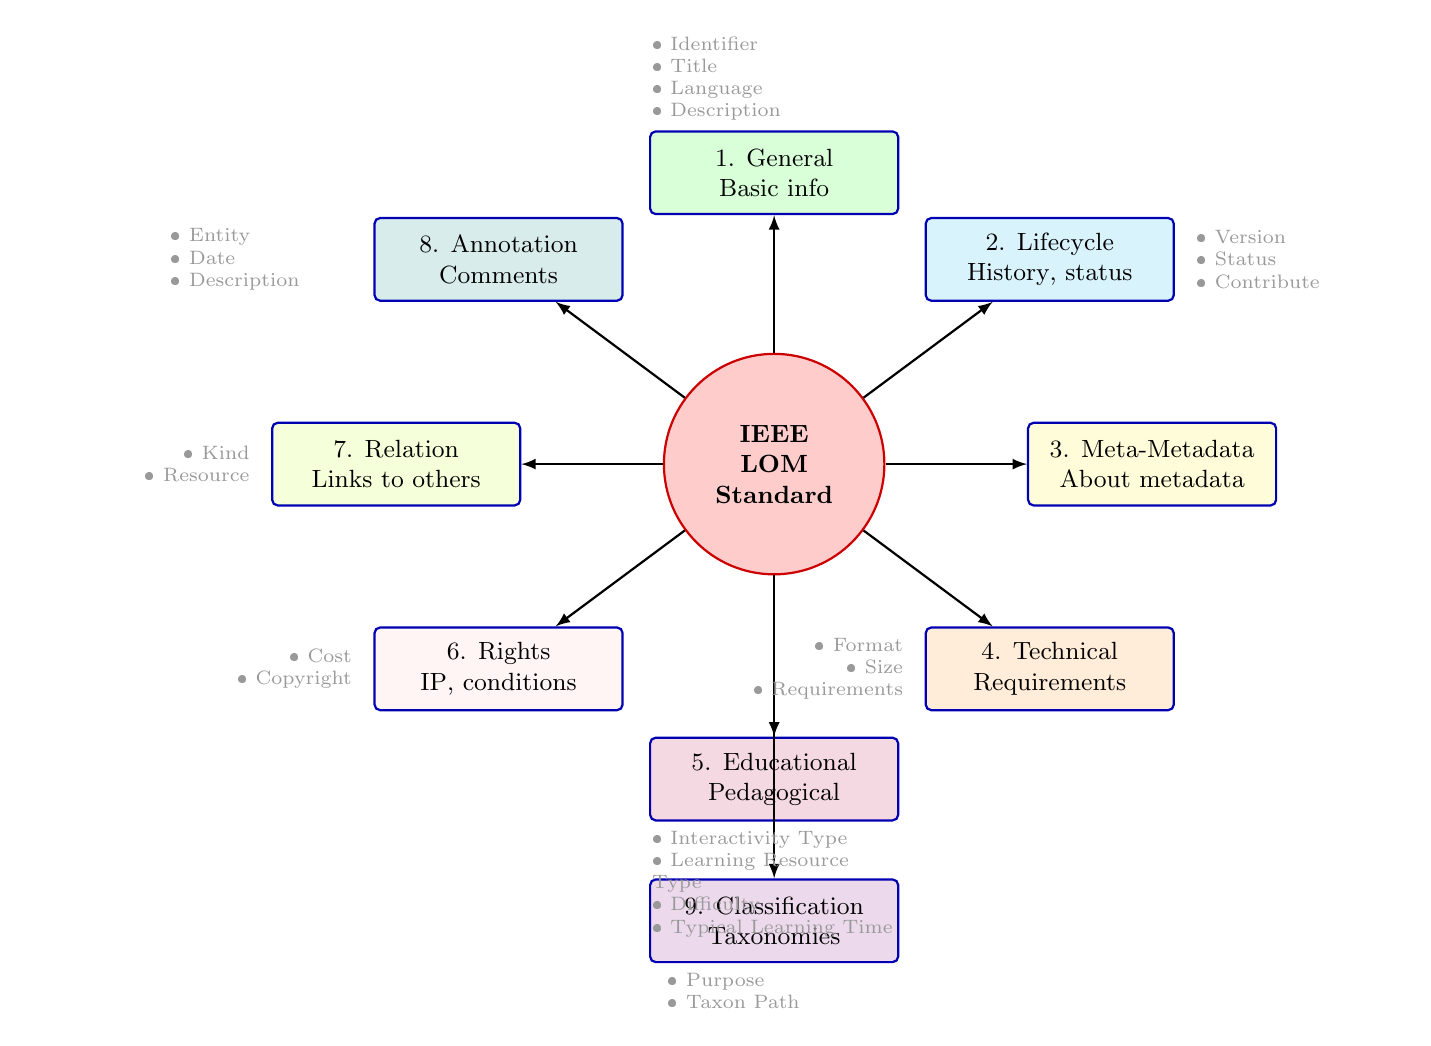
\begin{tikzpicture}[
    node distance=0.8cm and 1.5cm,
    every node/.style={font=\small},
    center/.style={circle, draw=red!80!black, fill=red!20, thick, minimum size=2.8cm, align=center, font=\small\bfseries},
    category/.style={rectangle, draw=blue!70!black, fill=blue!15, thick, minimum width=3.15cm, minimum height=1.05cm, rounded corners=2pt, align=center},
    arrow/.style={->, >=latex, thick}
]

% Center: IEEE LOM
\node[center] (lom) at (0,0) {\ENG{IEEE}\\\ENG{LOM}\\\ENG{Standard}};

% Categories arranged in a circle
\node[category, fill=green!15] (general) at (0, 3.7) {1. \ENG{General}\\\ENG{Basic} \ENG{info}};
\node[category, fill=cyan!15] (lifecycle) at (3.5, 2.6) {2. \ENG{Lifecycle}\\\ENG{History}, \ENG{status}};
\node[category, fill=yellow!15] (metameta) at (4.8, 0) {3. \ENG{Meta-Metadata}\\\ENG{About} \ENG{metadata}};
\node[category, fill=orange!15] (technical) at (3.5, -2.6) {4. \ENG{Technical}\\\ENG{Requirements}};
\node[category, fill=purple!15] (educational) at (0, -4.0) {5. \ENG{Educational}\\\ENG{Pedagogical}};
\node[category, fill=pink!15] (rights) at (-3.5, -2.6) {6. \ENG{Rights}\\\ENG{IP}, \ENG{conditions}};
\node[category, fill=lime!15] (relation) at (-4.8, 0) {7. \ENG{Relation}\\\ENG{Links} \ENG{to} \ENG{others}};
\node[category, fill=teal!15] (annotation) at (-3.5, 2.6) {8. \ENG{Annotation}\\\ENG{Comments}};

% 9th category in the middle-bottom
\node[category, fill=violet!15] (classification) at (0, -5.8) {9. \ENG{Classification}\\\ENG{Taxonomies}};

% Arrows from center to categories
\draw[arrow] (lom) -- (general);
\draw[arrow] (lom) -- (lifecycle);
\draw[arrow] (lom) -- (metameta);
\draw[arrow] (lom) -- (technical);
\draw[arrow] (lom) -- (educational);
\draw[arrow] (lom) -- (rights);
\draw[arrow] (lom) -- (relation);
\draw[arrow] (lom) -- (annotation);
\draw[arrow] (lom) -- (classification);

% Example elements for each category (annotations)
\node[font=\scriptsize, align=left, anchor=south, text width=3.1cm] at (general.north) {
    \textcolor{gray!80}{• \ENG{Identifier}}\\
    \textcolor{gray!80}{• \ENG{Title}}\\
    \textcolor{gray!80}{• \ENG{Language}}\\
    \textcolor{gray!80}{• \ENG{Description}}
};

\node[font=\scriptsize, align=left, anchor=west, text width=2.5cm] at ([xshift=0.15cm]lifecycle.east) {
    \textcolor{gray!80}{• \ENG{Version}}\\
    \textcolor{gray!80}{• \ENG{Status}}\\
    \textcolor{gray!80}{• \ENG{Contribute}}
};

\node[font=\scriptsize, align=right, anchor=east, text width=2.5cm] at ([xshift=-0.15cm]technical.west) {
    \textcolor{gray!80}{• \ENG{Format}}\\
    \textcolor{gray!80}{• \ENG{Size}}\\
    \textcolor{gray!80}{• \ENG{Requirements}}
};

\node[font=\scriptsize, align=left, anchor=north, text width=3.1cm] at (educational.south) {
    \textcolor{gray!80}{• \ENG{Interactivity} \ENG{Type}}\\
    \textcolor{gray!80}{• \ENG{Learning} \ENG{Resource} \ENG{Type}}\\
    \textcolor{gray!80}{• \ENG{Difficulty}}\\
    \textcolor{gray!80}{• \ENG{Typical} \ENG{Learning} \ENG{Time}}
};

\node[font=\scriptsize, align=right, anchor=east, text width=2.5cm] at ([xshift=-0.15cm]rights.west) {
    \textcolor{gray!80}{• \ENG{Cost}}\\
    \textcolor{gray!80}{• \ENG{Copyright}}
};

\node[font=\scriptsize, align=right, anchor=east, text width=2.7cm] at ([xshift=-0.15cm]relation.west) {
    \textcolor{gray!80}{• \ENG{Kind}}\\
    \textcolor{gray!80}{• \ENG{Resource}}
};

\node[font=\scriptsize, align=left, anchor=east, text width=2.3cm] at ([xshift=-0.15cm]annotation.west) {
    \textcolor{gray!80}{• \ENG{Entity}}\\
    \textcolor{gray!80}{• \ENG{Date}}\\
    \textcolor{gray!80}{• \ENG{Description}}
};

\node[font=\scriptsize, align=left, anchor=north, text width=2.7cm] at (classification.south) {
    \textcolor{gray!80}{• \ENG{Purpose}}\\
    \textcolor{gray!80}{• \ENG{Taxon} \ENG{Path}}
};

\end{tikzpicture}
\end{chapterfigurebox}
\caption{Οι εννέα κατηγορίες του \ENG{IEEE} \ENG{LOM} \ENG{Standard}. Κάθε κατηγορία περιέχει συγκεκριμένα \ENG{elements} που περιγράφουν διαφορετικές πτυχές του \ENG{learning} \ENG{object}: από γενικές πληροφορίες (\ENG{General}) μέχρι παιδαγωγικά χαρακτηριστικά (\ENG{Educational}) και τεχνικές απαιτήσεις (\ENG{Technical}).}
\label{fig:scorm12_lom_categories}
\end{figure}
